%placeholder
\section{DUNE Calibration Strategy}
\label{sec:phys-calib-strat}


The DUNE \dword{fd} presents a unique challenge for calibration in many ways. It differs from existing \dword{lbl} neutrino detectors and existing \dwords{lartpc} because of its size -- the largest \dword{lartpc} ever constructed -- but also because of its deep underground location. 
The DUNE \dword{nd}, which we expect to include a \dword{lartpc}, will also differ from previous experiments (e.g., MINOS and \nova). In particular, while the ND will be highly capable, pile-up and readout will be different, and this may complicate extrapolation of all relevant detector characteristics.

As for any \lartpc, full exploitation of DUNE's capability for precision tracking and calorimetry requires a detailed understanding of the detector response. The inherently highly convolved detector response model and the strong correlations that exist between various calibration quantities make this challenging. 
For example, the determination of energy associated with an event of interest will depend on the simulation model, associated calibration parameters, non-trivial correlations between the parameters, and spatial and temporal dependence of those parameters caused by the non-static nature of the \dword{fd}. 
Changes can be abrupt (e.g., noise, a broken resistor in the \dword{fc}), or ongoing (e.g., exchange of fluid through volume, ion accumulation).

Convincing physics measurements will require a demonstration that the overall detector response is well understood. The systematic uncertainties for the \dword{lbl} and low-energy (\dword{snb}) program will determine the required precision on dedicated calibration systems.
The calibration program must provide measurements at the few-percent-or-better level stably across an enormous volume and over a long period of time, and provide sufficient redundancy.

This section describes the current calibration strategy for DUNE that uses existing sources of particles, external measurements, and dedicated external calibration hardware systems. Existing calibration sources for DUNE include beam or atmospheric neutrino-induced samples, cosmic rays, argon isotopes, and instrumentation devices such as \lar purity and temperature monitors. Dedicated calibration hardware systems currently include laser and pulsed neutron system (PNS).
%and radioactive source deployment systems. %%KM removed
The responsibility of these hardware systems and assessment of alternative calibration system designs fall under the joint \dword{sp} and \dword{dp} calibration consortium. External measurements by \dword{protodune} and SBN will validate techniques, tools and the design of systems applicable to the DUNE calibration program;  \dword{protodune} will also perform essential measurements of charged particle interactions in \dword{lar}.

Under current assumptions, the calibration strategy described in this document is applicable to both \dwords{spmod} and \dwords{dpmod}. 
Section~\ref{sec:phys-calib-req} briefly describes the physics-driven calibration requirements. 
The nominal \dword{dune} \dword{fd} calibration design is described in Section~\ref{sec:phys-calib-sources}. Finally,
%Section~\ref{sec:phys-calib-sum} provides a summary along with future plans for calibration.
Section \ref{sec:phys-calib-approach} describes a staging plan for calibration
%the calibration development plan 
from after the \dword{tdr} through to the operation of the experiment including design validation at \dword{protodune}.



%%%%%%%%%%%%%%%%%%%%%%%%%%%%%%%%%%%%%%%%%%%%%%%%%%%%%%%


\subsection{Physics-driven Calibration Requirements}
\label{sec:phys-calib-req}


To perform adequate calibrations the physics processes that lead to the formation of the signals required for DUNE's broad physics program,
expected (and unexpected) detector effects must be carefully understood, as they ultimately affect the detector's energy, position and particle identification response. 
Other categories of effects, such as the neutrino interaction model or reconstruction pathologies, can impact measurements of physical quantities. These other effects are beyond the scope of the \dword{fd} calibration effort and would only lead to a higher overall error budget.

\subsubsection{\dword{lbl} physics}
\label{sec:phys-calib-lbl}

Calibration information needs to provide an approximately 1-2\% understanding of normalization 
and position resolution within the detector to support \dword{dune} \dword{lbl} physics. 
%Later studies expanded the simple treatment of energy  presented above. In particular, \num{1}\% 
A bias on the lepton energy has a significant impact on the sensitivity to \dword{cpv}. 
%
A \num{3}\% bias in the hadronic state (excluding neutrons) is important, as the inelasticity  distribution for neutrinos and antineutrinos is quite different.  Different fractions of their energies go into the hadronic state. Finally, while studies largely consider a single, absolute energy scale, DUNE will need to monitor and correct relative spatial differences across the enormous DUNE \dword{fd} volume; this is also true for time-dependent changes~\cite{ebias}.

A number of in situ calibration sources will be required to address these broad range of requirements. 
Michel electrons, neutral pions and radioactive sources (both intrinsic and external) are needed for calibrating detector response to electromagnetic activity in the tens-to-hundreds of MeV energy range. Stopping protons and muons from cosmic rays or beam interactions form an important calibration source for calorimetric reconstruction and particle identification. 
\Dword{protodune}, as a dedicated test beam experiment, provides important measurements to characterize and validate particle identification strategies in a \SI{1}{kt}-scale detector and is an essential input to the overall program. Dedicated calibration systems, like lasers, will be useful to provide in situ full-volume measurements of \efield distortions. 
Measuring the strength and uniformity of the \efield is a key aspect of calibration, as  estimates of calorimetric response and \dword{pid} depend on the \efield through recombination. The stringent physics requirements on energy scale and fiducial volume also put similarly stringent requirements on detector physics quantities such as \efield, drift velocity, electron lifetime, and the time dependencies of these quantities; this is discussed in more detail in 
the dedicated laser system discussion under Section~\ref{sec:phys-calib-hardware}.

\subsubsection{\dword{snb} and low-energy neutrino physics}
A combination of 6~MeV (direct neutron capture response), 9~MeV (peak visible $\gamma$-energy of interest to \dword{snb} and $^{8}B$/hep solar neutrinos), 15~MeV (upper visible energy of $^{8}B$/hep solar neutrinos) and $\sim$30~MeV (decay electrons) is needed to map the low energy response. Supernova signal events present specific reconstruction and calibration challenges, and observable energy is shared between different charge clusters and types of energy depositions. In particular, the supernova signal will have a low-energy electron, gamma and neutron capture component, and each needs to be characterized. As discussed further in Section~\ref{ch:snb-lowe}, primary requirements for this physics include 
(1) calibration of absolute energy scale and energy resolution, which is important for resolving spectral features of \dword{snb} events;
(2) calibration of time and light yield response of optical photon detectors;  
(3) absolute timing of events;  
(4) measurement of trigger efficiency at low energies;  and 
(5) understanding of detector response to radiological backgrounds. Further details on the necessary energy scale, energy resolution and trigger efficiency targets needed can be in Ref~\cite{bib:docdb14068}.
Potential calibration sources in this energy range include Michel electrons from muon decays (successfully utilized by ICARUS and \dword{microboone}~\cite{Acciarri:2017sjy}), which have a well known spectrum up to $\sim\,$\SI{50}{\MeV}.
Photons from neutral pion decay (from atmospheric and beam induced $\pi^0$) will provide an overall energy scale between \SI{50}{\MeV} and \SI{100}{\MeV}, in addition to cosmic ray muon energy loss. 
However, the limited statistical power of those samples (see Table~\ref{tab:cosmic-ray-calib-rates}) mean that it is not possible for these samples to provide the energy scale or resolution at the spatial and temporal granularity needed.
The pulsed neutron system can provides a source of direct neutron capture across the entire DUNE volume, providing a timing and energy calibration.
%removing the laser part here since not relevant?
%the laser system is timed as well. 
The proposed radioactive source system provides an in situ source of the electrons and de-excitation $\gamma$ rays, which are directly relevant for physics signals from \dword{snb} or $^{8}B$ solar neutrinos. These two systems (discussed in more detail in Section~\ref{sec:phys-calib-hardware}) can provide calibrations of photon, electron, and neutron response for energies below \SI{10}{\MeV}, where photons and electrons may have very different characteristics in \dword{lar}.


\subsubsection{Nucleon decay and other exotic physics}
The calibration needs for nucleon decay and other exotic physics are comparable to those for the \dword{lbl} program, as listed in Section~\ref{sec:phys-calib-lbl}. Signal channels for light \dword{dm} and sterile neutrino searches will be \dword{nc} interactions that are background to the \dword{lbl} physics program. 
Based on the widths of $dE/dx$-based metrics of \dword{pid}, qualitatively, we need to calibrate $dE/dx$ across all drift and track orientations at the few-percent level, similar to the \dword{lbl} effort.





\subsection{Calibration Sources, Systems and External Measurements}
\label{sec:phys-calib-sources}
%\subsubsection{Calibration sources and systems}
Calibration sources and systems provide measurements of the detector response model parameters, or provide tests of the response model itself. Calibration measurements can also provide corrections to data, data-driven efficiencies, systematics and particle responses. 
Figure~\ref{fig:calibneeds} shows the broad range of categories of measurements that calibrations can provide, and lists 
%the critical 
important calibration parameters for DUNE's detector response model applicable to both \dword{sp} or \dword{dp}. Due to the significant interdependencies of many parameters (e.g., recombination, \efield, and \lar purity), a calibration strategy will either need to  measure parameters iteratively, or find sources that break these correlations.

Table~\ref{tab:calibsystem} provides a list of the calibration sources and dedicated calibration systems, along with their primary usage, that will comprise the current
%currently envisioned 
nominal DUNE \dword{fd} calibration design. 
The next sections provide more details on each of them. \Dword{protodune} and previous measurements provide independent tests of the response model, indicating that the choice of parameterization and values correctly reproduces real detector data. 
Not all of the ex situ measurements can be directly extrapolated to DUNE, however, due to other detector effects and conditions -- only those considered to be universal (e.g., argon ionization energy). 

Each of the many existing calibration sources comes with its own challenges. For example, while electrons from muon decay (Michel electrons) are very useful for studying the detector response to low-energy electrons (\SI{50}{\MeV}), these low-energy electrons present reconstruction challenges due to the loss of charge from radiative photons, as demonstrated in \dword{microboone}~\cite{Acciarri:2017sjy}.  
Michel electrons are therefore considered an important, independent, and necessary test of the TPC energy response model, but they will not provide a measurement of a particular response parameter.

\begin{dunefigure}[Categories of measurements provided by calibration]{fig:calibneeds}{Categories of measurements provided by calibration.}
%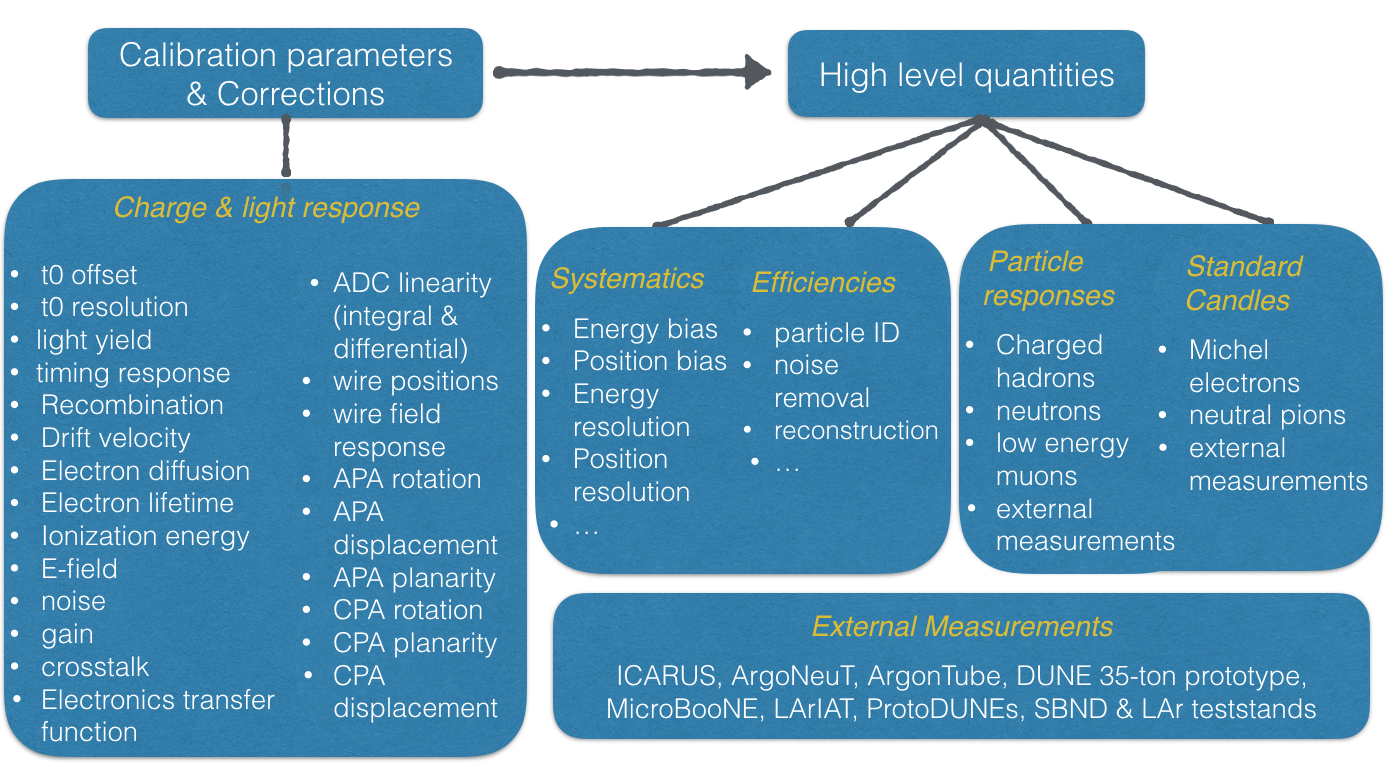
\includegraphics[width=.9\textwidth]{graphics/CalibNeeds_Final.png}
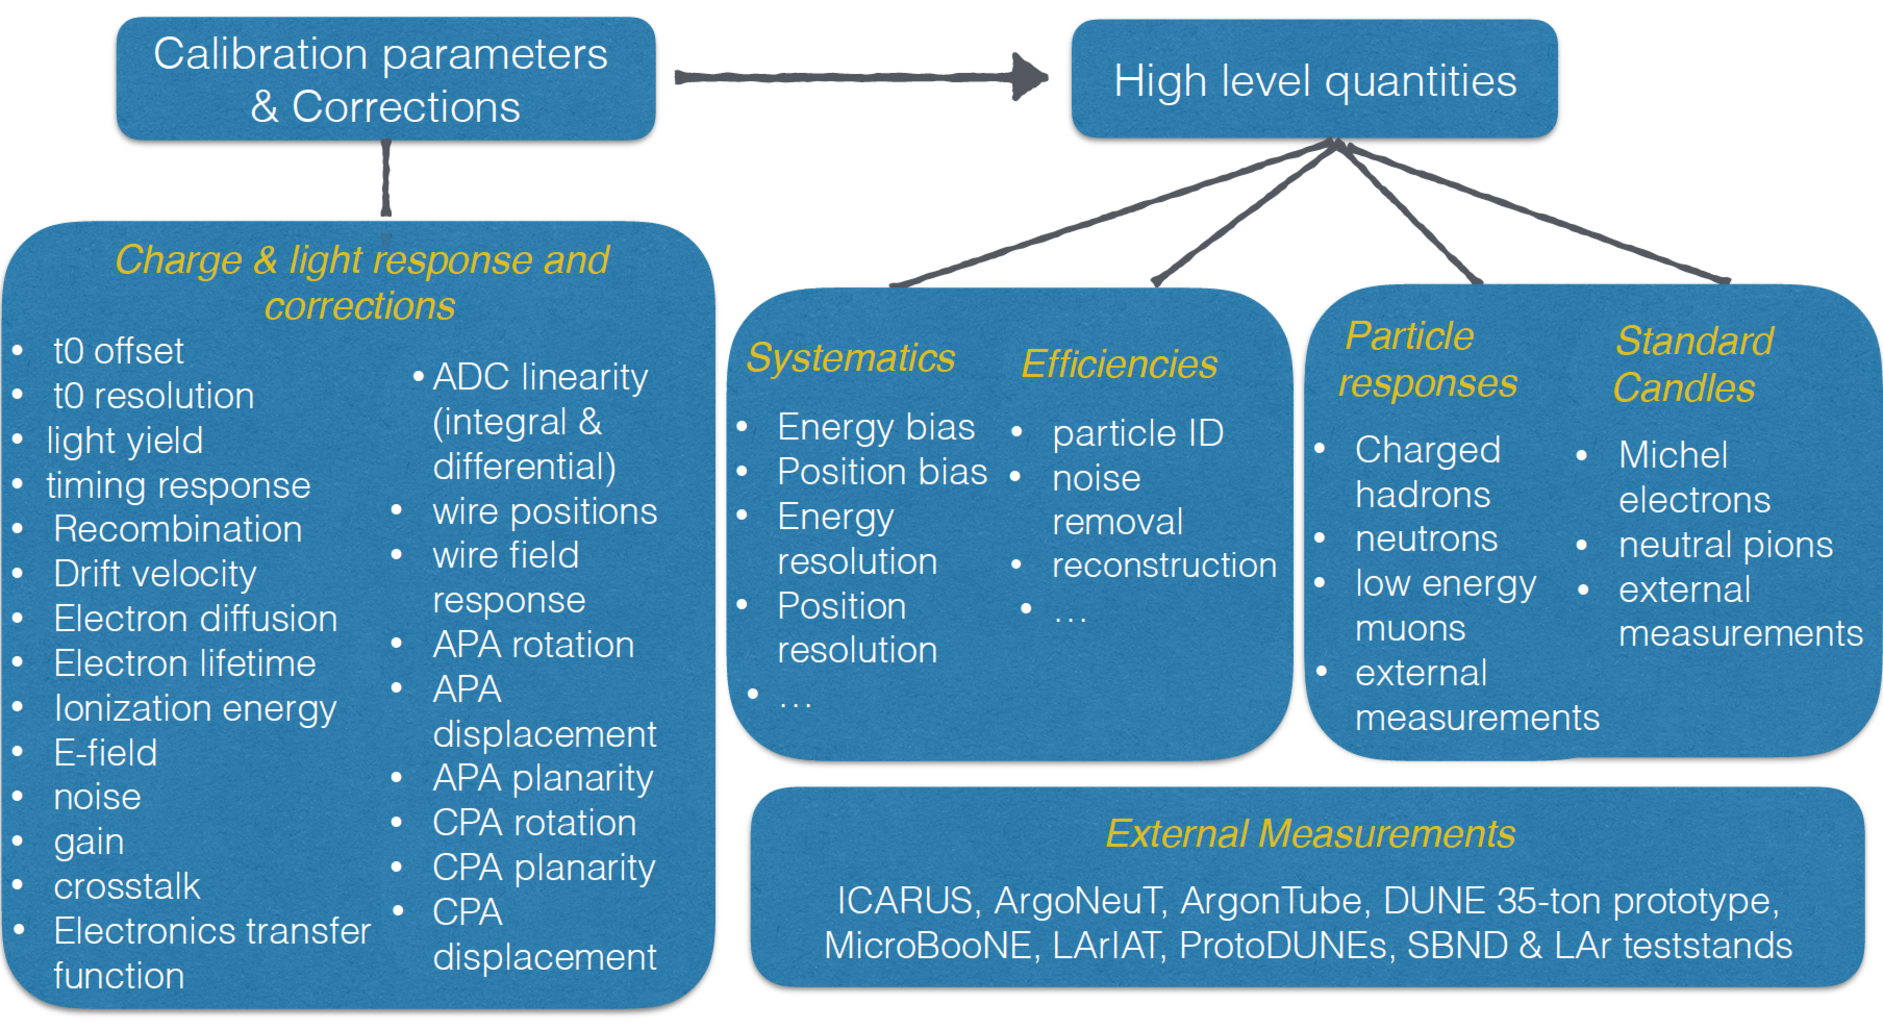
\includegraphics[width=.9\textwidth]{graphics/CalibNeedsFig_TDR_cropped.pdf}
\end{dunefigure}

\begin{dunetable}[Calibration systems and sources of the nominal DUNE FD calibration design]
{p{.4\textwidth}p{.55\textwidth}}{tab:calibsystem}{Primary calibration systems and sources that comprise the nominal DUNE FD calibration design along with their primary usage.}
%{ll}
% &  \\ \textbf{Usage} \toprowrule
System & \textbf{Primary Usage}  \\ \toprowrule 
& \\
\textbf{Existing Sources} & \textbf{Broad range of measurements} \\ \toprowrule
$\mu$, predominantly from cosmic ray & Position (partial), angle (partial), %velocity (timing), 
electron lifetime, wire response, $dE/dx$ calibration etc.\\ \colhline % also timing offsets listed, related to drift velocity based on our discussion?
Decay electrons, $\pi^0$ from beam, cosmic, atm $\nu$ & Test of electromagnetic response model \\ \colhline
$^{39}$Ar beta decays &  electron lifetime (x,y,z,t), diffusion, wire response \\  \colhline
& \\ 
\textbf{External Measurements} & \textbf{Tests of detector model, techniques and systems} \\ \toprowrule
ArgoNeuT~\cite{Acciarri:2013met}, ICARUS~\cite{Amoruso:2004dy, Antonello:2014eha, Cennini:1994ha}, MicroBooNE & Model parameters (e.g., recombination, diffusion) \\ \colhline 
DUNE \dword{35t}~\cite{Warburton:2017ixr} & Alignment and \textit{t0} techniques\\ \colhline 
ArgonTUBE~\cite{Ereditato:2014tya}, MicroBooNE~\cite{Acciarri:2016smi}, SBND, ICARUS~\cite{Auger:2016tjc},  \Dword{protodune}~\cite{Abi:2017aow} & Test of systems (e.g., Laser) \\ \colhline
ArgoNeuT~\cite{Acciarri:2015ncl}, MicroBooNE~\cite{bib:uBlifetime, MICROBOONE-NOTE-1018-PUB, MICROBOONE-NOTE-1028-PUB, Acciarri:2017sjy, Abratenko:2017nki, Acciarri:2013met}, ICARUS~\cite{Ankowski:2008aa,  Ankowski:2006ts,Antonello:2016niy},  \Dword{protodune} & Test of calibration techniques and detector model (e.g., electron lifetime, Michel electrons, $^{39}$Ar beta decays) \\ \colhline
\Dword{protodune}, LArIAT~\cite{Cavanna:2014iqa}, CAPTAIN~\cite{Bhandari:2019rat} & Test of particle response models and fluid flow models \\  \colhline
\dword{lartpc} test stands~\cite{Cancelo:2018dnf, Moss:2016yhb, Moss:2014ota, Li:2015rqa} & Light and LAr properties; signal processing techniques \\ \colhline 
& \\
\textbf{Monitoring Systems} & \textbf{Operation, Commissioning and Monitoring} \\ \toprowrule
Purity monitors & Electron lifetime \\ \colhline
Photon detection monitoring System & \dword{pds} response \\ \colhline
Thermometers & Temperature, velocity; test of fluid flow model \\ \colhline
Charge injection & Electronics response \\ \colhline
& \\
\textbf{Dedicated Calibration Systems} & \textbf{Targeted (near) independent, precision calibration}\\ \toprowrule
Direct ionization via laser & Position, angle, electric field (x,y,z,t) \\ \colhline
Photoelectric ejection via laser & Position, electric field (partial) \\ \colhline
Neutron injection & Test of \dword{snb} signal, neutron capture model \\ \colhline
Proposed Radioactive source deployment & Test of \dword{snb} signal model \\ \colhline
%External Muon Tracker (if deployed) & Position, angle, muon reconstruction efficiency \\ \colhline
\end{dunetable}  


%%%%%%%%%%%%%%%%%%%%%%%%%%%%%%%%%%%%%%%%%%%%%%%%%%%%%%%

\subsubsection{Existing sources} 
\label{sec:phys-calib-exis}
Cosmic rays and neutrino-induced interactions provide commonly used ``standard candles,'' e.g., electrons from muon decays, and photons from neutral pions, which have characteristic energy spectra. Cosmic ray muons are also used to determine detector element locations (alignment), timing offsets or drift velocity, electron lifetime, and channel-by-channel response, and to help constrain \efield distortions. 
Table~\ref{tab:cosmic-ray-calib-rates} summarizes the rates for cosmic ray events. Certain measurements (e.g., channel-to-channel gain uniformity and cathode panel alignment) are estimated to take several months of data. Table~\ref{tab:atmos_rates} gives the atmospheric $\nu$ interaction rates, which  
 are comparable to beam-induced events -- neither occurs at sufficient rates to provide meaningful spatial or temporal calibration; they will likely provide supplemental measurements only. (The beam will not yet be operational for calibration of the first \dword{detmodule} during early data taking.) Instead, we can use the reconstructed energy spectrum of ${}^{39}$Ar beta decays to make a precise measurement of electron lifetime with spatial and temporal variations. 
 This can also provide other necessary calibrations, such as measurements of wire-to-wire response variations and diffusion measurements using the signal shapes associated with the beta decays. The ${}^{39}$Ar beta decay rate in commercially-provided argon is about \SI{1}{\becquerel\per\kilo\gram}, so $O(\mathrm{50k})$ ${}^{39}$Ar beta decays are expected in a single \SI{5}{\milli\s} event readout in an entire \nominalmodsize \detmodule. 
 The ${}^{39}$Ar beta decay cutoff energy is \SI{565}{\keV},  which is close to the energy deposited on a single wire by a \dword{mip}. However, several factors can impact the observed charge spectrum from ${}^{39}$Ar beta decays, such as electronics noise, electron lifetime and recombination fluctuations; more details can be found in the Appendix~\ref{app:ar39}. MicroBooNE~\cite{MICROBOONE-NOTE-1050-PUB} and ProtoDUNE are actively pursuing this technique, thus providing valuable inputs for DUNE.

\begin{dunetable}
[Annual rates for classes of cosmic-ray events useful for calibration]
{lrl}
{tab:cosmic-ray-calib-rates}
{Annual rates for classes of cosmic-ray events described in this section assuming 100\% reconstruction efficiency.  Energy, angle, and fiducial requirements
have been applied. Rates and geometrical features apply to the single-phase far detector design. }
Sample & Annual Rate & Detector Unit \\ \colhline
Inclusive & $1.3\times 10^6$ & Per \nominalmodsize module \\ \colhline
Vertical-Gap crossing & 3300 & Per gap \\ \colhline
Horizontal-Gap crossing & 3600 & Per gap \\ \colhline
\dword{apa}-piercing & 2200 & Per \dword{apa} \\ \colhline
\dword{apa}-\dword{cpa} piercing & 1800 & Per active \dword{apa} side \\ \colhline
\dword{apa}-\dword{cpa} piercing, \dword{cpa} opposite to \dword{apa} & 360 & Per active \dword{apa} side \\ \colhline
Collection-plane wire hits & 3300 & Per wire \\ \colhline
Stopping Muons & 28600 & Per \nominalmodsize module \\ \colhline
$\pi^0$ Production & 1300 & \nominalmodsize module \\ \colhline
\end{dunetable}

\subsubsection{Monitors} 
 
Chapter~8 of \voltitlesp{} and \voltitledp{} discuss several instrumentation and detector monitoring devices in detail. These devices, including liquid argon temperature monitors, \lar purity monitors, gaseous argon analyzers, cryogenic (cold) and inspection (warm) cameras, and liquid level monitors, will provide valuable information for early calibrations and for tracking the space-time dependence of the \dwords{detmodule}. 
The \dword{cfd} simulations play a key role for calibrations initially in the design of the cryogenics recirculation system, and later for physics studies when the cryogenics instrumentation data can be used to validate the simulations. Chapters~4 and~5 of the \dword{detmodule} volumes discuss other instrumentation devices essential for calibration, such as drift \dword{hv} current monitors and external charge injection systems. 

\subsubsection{External measurements} 

DUNE will use external measurements from past experimental runs (e.g., ArgoNeuT, the DUNE \dword{35t}, ICARUS, and \lariat), from ongoing and future experiments (e.g., \dword{microboone}, \dword{protodune}, and SBND), and from small scale \dword{lartpc} test stands. External measurements provide a test bed for dedicated calibration hardware systems and techniques for the \dword{fd}. In particular, \dword{protodune} will provide validation of the fluid flow model using cryogenic instrumentation data. 
Early calibration for physics in DUNE will utilize \lar physical properties from \Dword{protodune} or SBN  for tuning detector response models in simulation. Table~\ref{tab:calibsystem} provides  references for specific external measurements. The usability of ${}^{39}$Ar has been demonstrated with \microboone data~\cite{MICROBOONE-NOTE-1050-PUB}. 
Use of  ${}^{39}$Ar  and other radiological sources and, in particular, the \dword{daq} readout challenges associated with their use, will be tested on the \dword{protodune} detectors. Dedicated systems for DUNE, 
including the laser system, have been used by previous experiments (ARGONTUBE~\cite{Zeller:2013sva,Ereditato:2014lra}, CAPTAIN, and MicroBooNE experiments) and at SBND in the future, and will provide more information on use of the system and optimization of the design.  The small-scale \lar test stand planned at Brookhaven National Lab, USA, will provide important information on simulation and calibration of field response for DUNE.

External measurements of particle response (e.g. pion interactions in \dword{lar}) are also important inputs to the detector model. These include dedicated measurements made with ProtoDUNE, LArIAT, and CAPTAIN~\cite{Bhandari:2019rat}; the DUNE ND, with both a \dword{lar} and low density gas detector, will also make measurements which characterize the relevant cross sections and outgoing final state particles.

%%%%%%%%%%%%%%%%%%%%%%%%%%%%%

\subsubsection{Dedicated Calibration Hardware Systems}
\label{sec:phys-calib-hardware}

This section briefly describes the physics motivation and measurement goals for the calibration hardware systems and the designs currently envisioned. The calibration chapters in \voltitlesp{} and \voltitledp{} of the \dword{tdr} provide further details on the design and development plan for these systems. We plan to deploy prototype designs of these systems in 
%a potential 
the phase 2 of \dword{protodune} to demonstrate proof-of-principle.

\textbf{Laser systems} 

The primary purpose of a laser system is to provide an independent, fine-grained estimate of the \efield in space or time, which is a critical parameter for physics signals as it ultimately impacts the spatial resolution and energy response of the detector. External measurements, e.g.,  MicroBooNE's, use both a laser system and cosmic rays to estimate the \efield, however the expected cosmic rate at the deep underground installation of the \dword{fd} will not provide sufficient spatial or temporal granularity to study local distortions.

\efield distortions can arise from multiple sources. Current simulation studies indicate that positive ion accumulation and drift (space charge) due to ionization sources such as cosmic rays or ${}^{39}$Ar are small in the \dword{fd}; however, the fluid flow pattern in the \dword{fd} is not yet sufficiently understood to exclude the possibility of stable eddies that may amplify the effect for both \single and \dual modules. The \dword{dpmod} risks significant further amplification due to  accumulation in the liquid of ions created by the electron multiplication process in the gas phase.
%SG: above sentence is a direct edit from Bo
%due to ion accumulation at the liquid-gas interface. 
Detector imperfections can also cause localized \efield distortions. Examples include \dword{fc} resistor failures, non-uniform resistivity in the voltage dividers, \dword{cpa} misalignment, \dword{cpa} structural deformations, and \dword{apa} and \dword{cpa} offsets and  deviations from flatness. Individual \efield distortions may add in quadrature with other effects, and can reach 4-5\% under certain conditions, which corresponds to a 1-2\% impact on charge, 
%(dQ), 
and a $\sim 2$ cm impact on position (and fiducial volume). Both charge and position distortions affect energy scale. Understanding all these effects requires an in situ calibration of the E field with a precision of about 1\% with a coverage of at least 75\% of the detector volume.
%proper in situ calibration of the \efield{}. 

The laser calibration system offers secondary uses, e.g., alignment (especially modes that are weakly constrained by cosmic rays, see Figure~\ref{fig:apacurtainalign}), stability monitoring, and diagnosing detector failures in systems such as \dword{hv}.  

\begin{dunefigure}[Sample distortion that may be difficult to detect with cosmic rays]{fig:apacurtainalign}
{An example of a distortion that may be difficult to detect with cosmic rays.  The \dword{apa} frames are shown as rotated rectangles, as viewed from the top.}

\includegraphics[width=0.8\textwidth]{graphics/apacurtainalign.png}
\end{dunefigure}

Two systems are under consideration to extract the \efield map: \phel{}s from the \lartpc cathode and direct ionization of the \dword{lar}, both driven by a \SI{266}{\nano\m} laser.  The reference design from \dword{microboone}~\cite{bib:uBlaser2019} and SBND uses direct ionization laser light with multiple laser paths. This can provide field map information in $(x, y, z, t)$; a \phel laser only provides an integrated measurement of the \efield along the drift direction.
The ionization-based system can characterize the \efield with fewer dependencies compared to other systems. If two laser tracks enter the same spatial voxel in a \dword{detmodule}, the relative position of the tracks provides an estimate of the local \threed \efield. The deviation from straightness of single ``laser tracks'' can also be used to constrain local \efield{}s. Comparison of the known laser track path against the path reconstructed from cosmic or beam data, assuming uniform \efield, can also be used to estimate local \efield distortions. A schematic of the ionization laser setup and a laser track from \dword{microboone} is shown in Figure~\ref{fig:uB_laser_schematic}.


\begin{dunefigure}[\microboone laser calibration system schematics]{fig:uB_laser_schematic}
{Left: Schematics of the ionization laser system in \dword{microboone}~\cite{Antonello:2015lea}. Right: A UV laser event in the MicroBooNE detector~\cite{bib:uBlaser2019}. The laser track can be identified by the endpoint on the cathode (larger charge visible at the top of the image) and the absence of charge fluctuations along the track. The charge released at the cathode comes from photoelectric effect. Other tracks seen in the display are from cosmic muons.}
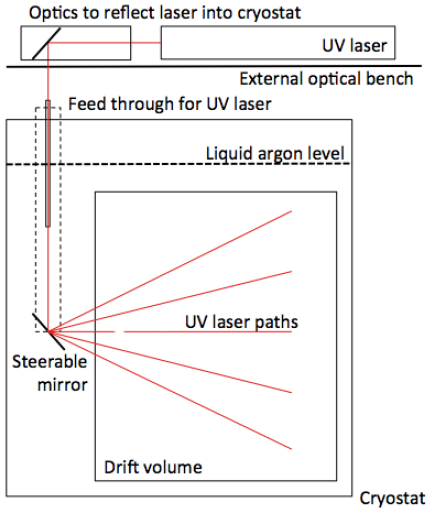
\includegraphics[width=0.45\linewidth]{graphics/uB_laser_schematic}
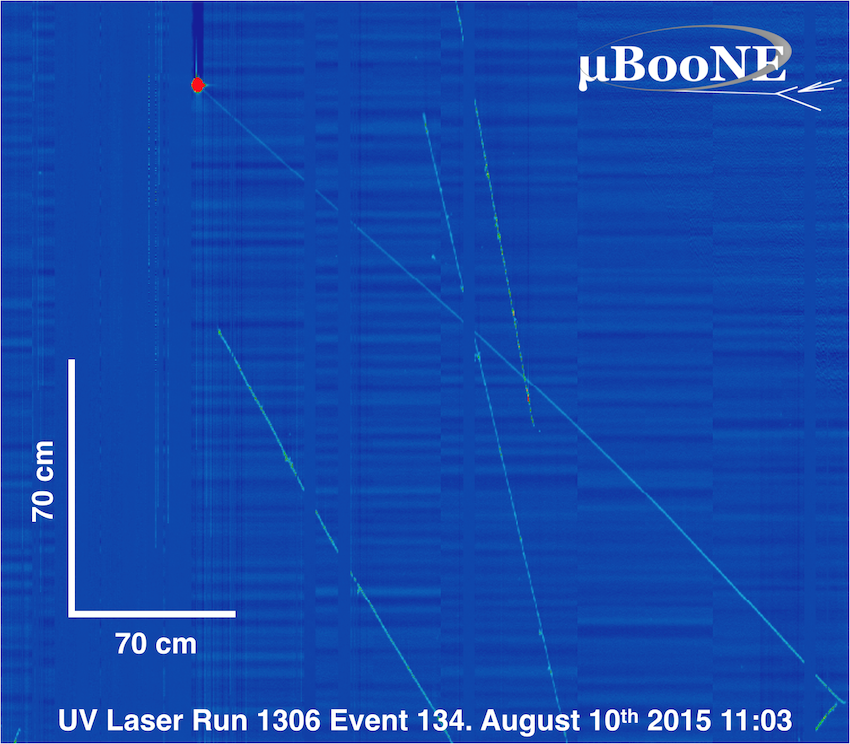
\includegraphics[width=0.45\linewidth]{graphics/run1306_ev134-2.png}
\end{dunefigure}
%\fixme{should \cite{ref:ub-laser-event} be \cite{bib:uBlaser2019}? Anne}

A \phel{}-based calibration system was used in the T2K gaseous (predominantly Ar), TPCs~\cite{Abgrall:2010hi}. 
Thin metal surfaces placed at surveyed positions on the cathode provided point-like and line sources of \phel{}s when illuminated by a laser. The T2K \phel system provided measurements 
of adjacent electronics modules' relative timing response, drift velocity with a few \si{\nano\s} resolution over their \SI{870}{\milli\m} drift distance, electronics gain, 
transverse diffusion, and an integrated measurement of the \efield along the drift direction. DUNE would use the system similarly to diagnose electronics or TPC response issues on demand, and to provide an integral field measurement across drift as well as measure relative distortions of $y$, $z$ positions with time, $x$ and/or drift velocity. \microboone has also observed ejection of \phel{}s from the cathode using the direct ionization laser system. 

\textbf{Pulsed neutron source} 

An external neutron generator system would provide a triggered, well defined energy deposition from neutron capture in $^{40}$Ar detectable throughout the \dword{detmodule} volume. Neutron capture is a critical component of signal processes for \dword{snb} and \dword{lbl} physics; this system would enable direct testing of the detector response  spatially and temporally for the low-energy program.  This is important to measure energy scale, energy resolution and detection threshold spatially and temporally across the enormous DUNE volume.

\begin{dunefigure}[Cross sections enabling the PNS concept]{fig:pns_xsec}
{Illustration of interference anti-resonance dip in the cross section of  \isotope{Ar}{40}. Elastic scattering cross section data is obtained from ENDF VIII.0}
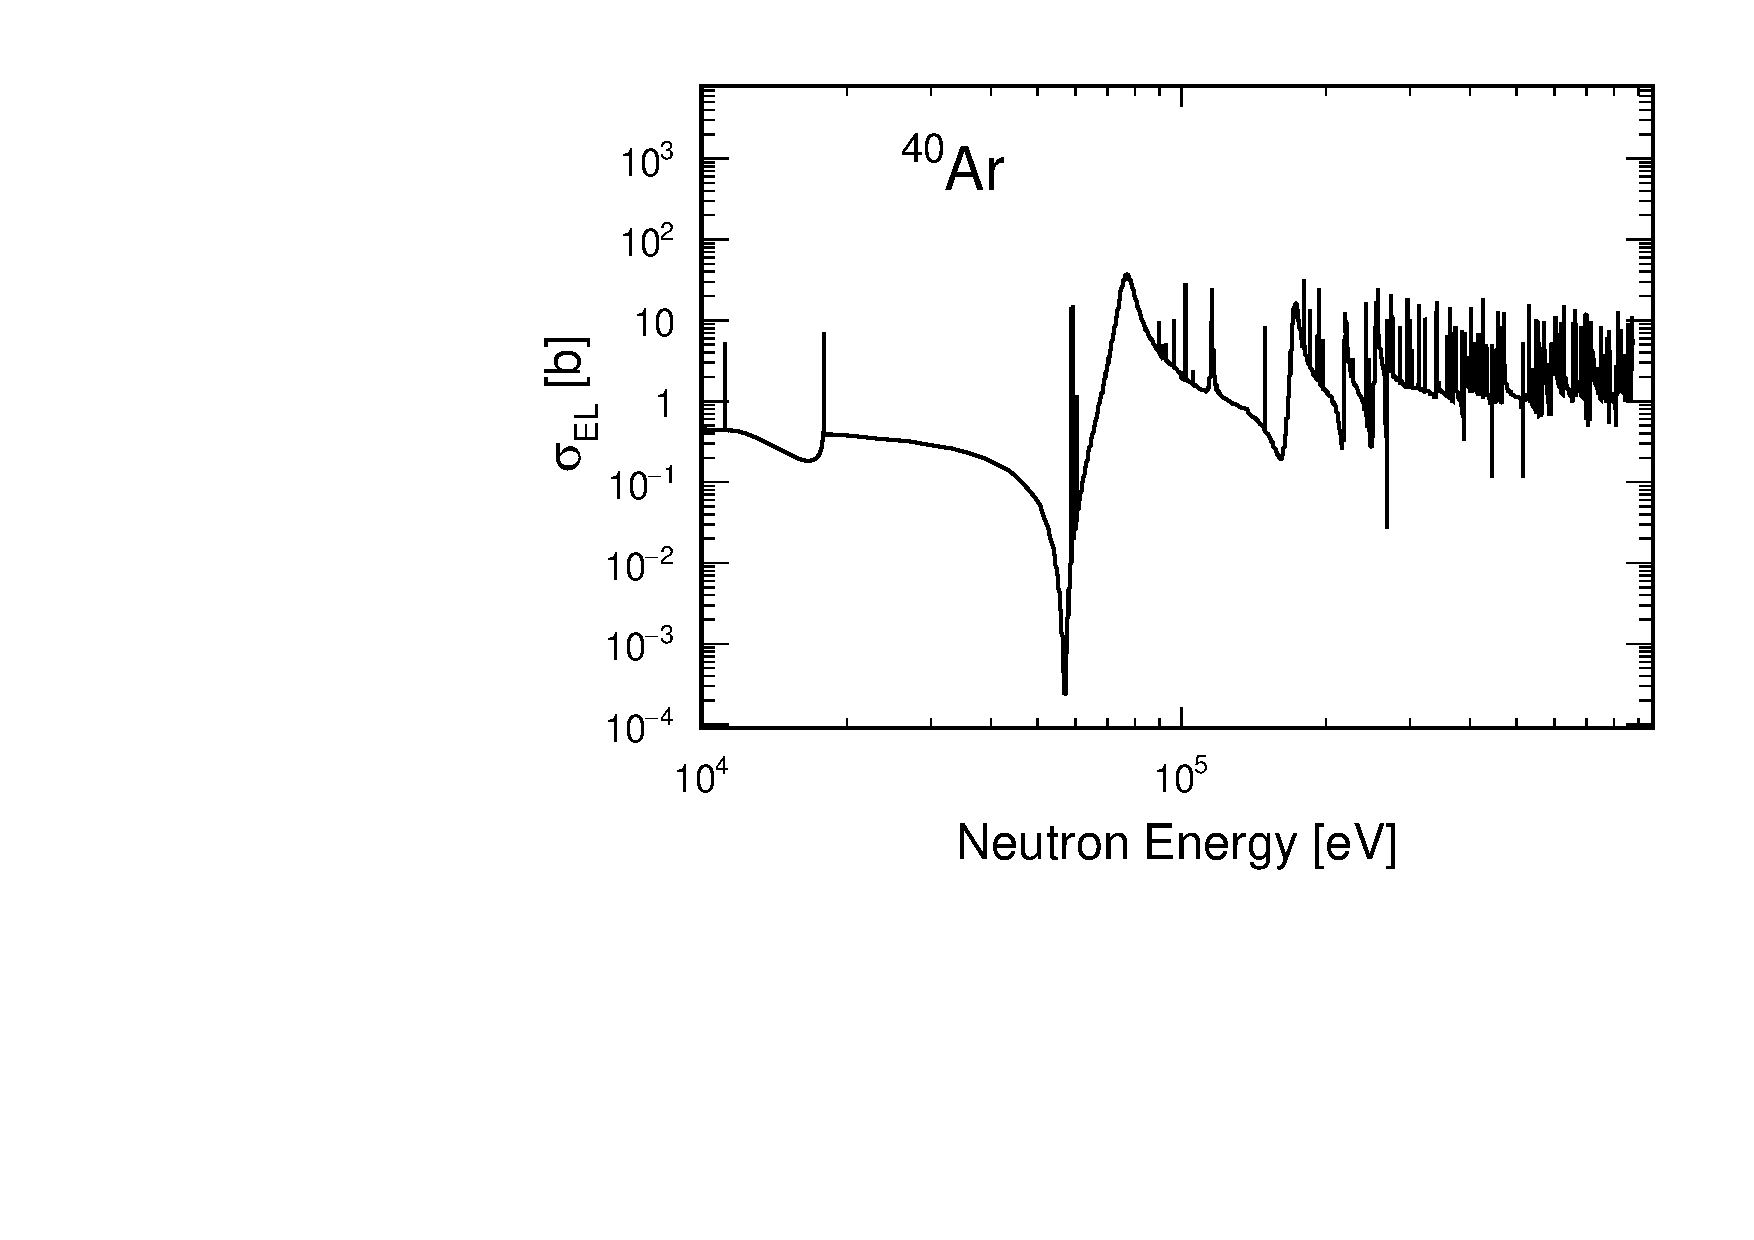
\includegraphics[width=8cm]{graphics/Calib_pns_ES_xsec_Ar40.pdf}
\end{dunefigure}

A triggered pulse of neutrons can be generated outside the TPC and injected into the \dword{lar}, where it spreads through the entire volume to produce a mono-energetic cascade of photons via the $^{40}$Ar(n,$\gamma$)$^{41}$Ar capture process. The uniform population of neutrons throughout the \dword{detmodule} volume exploits a remarkable property of argon -- the near transparency to neutrons of energy near \SI{57}{\keV}. 
This is due to a deep minimum in the cross section caused by the destructive interference between two high-level states of the \isotope{Ar}{40} nucleus (see Fig.~\ref{fig:pns_xsec}). This cross section ``anti-resonance'' is approximately  \SI{10}{\keV} wide, and \SI{57}{keV} neutrons consequently have a scattering length of \SI{859}{m}; the scattering length averaged over the isotopic abundance in natural Ar is approximately \SI{30}{m}. 
For neutrons moderated to this energy the DUNE \dword{lartpc} is essentially transparent. The \SI{57}{keV} neutrons that do scatter quickly leave the anti-resonance and thermalize, at which time they capture. Each neutron capture releases exactly the binding energy difference between \isotope{Ar}{40} and \isotope{Ar}{41}, about \SI{6.1}{\MeV}, in the form of gamma rays. 
The neutron capture cross-section and the $\gamma$ spectrum have been measured and characterized. Recently, the ACED Collaboration performed a neutron capture experiment using  the Detector  for Advanced  Neutron  Capture  Experiments  at DANCE (ACED)  at the  Los  Alamos  Neutron  Science  Center  (LANSCE). The result of neutron capture cross-section was published~\cite{Fischer:2019qfr} and will be used to prepare a database for the neutron capture studies. The data analysis of the energy spectrum of correlated gamma cascades from neutron captures is underway.

DUNE plans
%would plan 
to place a fixed, shielded deuterium-deuterium ($DD$) neutron generator  above a penetration in the hydrogenous insulation of the \dword{detmodule} cryostat. Between the generator and the cryostat, layers of water or plastic and intermediate fillers would provide sufficient degradation of the neutron energy. 

\textbf{Additional Systems}

There are 
%alternative designs or 
additional systems under consideration for DUNE calibration. Radioactive source deployment provides an in situ source of low energy electrons and de-excitation gamma rays at a known location and with a known activity, which are directly relevant for detection of \dword{snb} or $^{8}B$ solar neutrinos. As shown in Section~\ref{ch:snb-lowe}, the electron and photon response in the TPC is quite different (electrons leave worm-like tracks, photons leave `blips'). The PNS source will provide a 6.1 MeV multi-photon signal; radioactive sources can provide a single photon signal to measure detection threshold and demonstrate sufficient uncertainty on energy resolution at the peak of the \dword{snb} photon signal.  The radioactive source system is under study, and feasibility and safety of deployment would be established with a dedicated run using a prototype system in ProtoDUNE.

The utility of internal source injection (e.g., ${}^{222}$Rn or ${}^{220}$Rn injection) for mapping electron lifetime and fluid flow in the \dword{tpc}, used in dark matter experiments, will also be considered in the future. The major challenge for this system is if the 
coverage of the \dword{pds} is sufficient, and whether or not it will be able to identify a signal and trigger over the massive amount of ${}^{39}$Ar present. Recognizing that the presence of radioactive impurities can also impact such a system, the newly formed DUNE \dword{fd} Background Task Force will address this concern. This system would not require any cryostat penetrations or affect major \dword{daq} requirements.





%%%%%%%%%%%%%%%%%%%%%%%%%%%%%%%%%%%%%%%%%%%%%%%%%%


\subsection{Calibration Staging Plan}
%\subsection{Calibration  Plan}
\label{sec:phys-calib-approach}

%\fixme{KM: I felt the previous summary was not really full of content, and that ending on seeing the entire system working was better.}

The calibration strategy for DUNE will need to address the evolving operational and physics needs at every stage of the experiment in a timely manner using the primary sources and systems listed in Table~\ref{tab:calibsystem}. 
Here we describe the validation plan for calibration systems at ProtoDUNE and a staging plan to deploy calibration systems during different phases of the experiment: commissioning, early data taking, and stable operations. 

This \dword{tdr} presents the baseline calibration systems and strategy. Post-\dword{tdr}, once the calibration strategy is set, the calibration consortium will need to develop the necessary designs for calibration hardware along with tools and methods to be used with various calibration sources. To allow for flexibility in this process, the physical interfaces for calibration such as flanges or ports on the cryostat will be designed to accommodate the calibration hardware. As described in the calibration \dword{sp} detector volume, the calibration task force has provided the necessary feedthrough penetration design 
%updates 
for the \dword{spmod} and will soon finalize the design for the \dword{dpmod}.  As DUNE physics turns on at different rates and times, a calibration strategy at each stage for physics and data taking is required. The strategy described in this section assumes that all systems are commissioned and deployed according to the nominal DUNE run plan.

\textit{Design Validation:} A second run of ProtoDUNE will be used to validate the designs of dedicated calibration systems, including the laser, PNS, and possibly the proposed radioactive source. In addition, ProtoDUNE data (and the SBN program) will provide data analysis techniques, tools, and detector model simulation improvements in advance of DUNE operation.


\textit{Commissioning:} When a \dword{detmodule} is filled, data from various instrumentation devices validate the argon fluid flow model and purification system. Once filled and at the desired high voltage, the \dword{detmodule} immediately becomes live for \dword{snb} and proton decay signals (beam and atmospheric neutrino physics will require a few years of data accumulation)
at which point it is critical that early calibration track the space-time dependence of the detector. Noise data 
and pulser data (taken with signal calibration pulses injected into the electronics) are needed to understand the TPC electronics response. Essential systems at this stage include temperature monitors, purity monitors, \dword{hv} monitors, robust \dword{fe} charge injection system for cold electronics, and a \dword{pds} monitoring system. 
In addition, as the $^{39}$Ar data is available immediately, DUNE must be ready (in terms of reconstruction tools and methods) to utilize $^{39}$Ar decays for understanding both low-energy response and space-time uniformity. 
Dedicated calibration systems as listed in Table~\ref{tab:calibsystem} are deployed and commissioned at this stage. Commissioning data from these systems must verify the expected configuration for each system and identify any needed adjustments to tune for data taking.

\textit{Early data taking:} Since DUNE will not yet have all in situ measurements of \lar physical properties at this stage, early calibration of the detector will use \lar measurements from \dword{protodune} or SBN, and \efield{}s from calculations tuned to measured \dword{hv} values.
This early data will most likely need to be recalibrated at a later stage with dedicated calibration runs when in situ measurements are available and as data taking progresses. 
The early physics will also require analysis of cosmic ray muon data to develop methods and tools for muon reconstruction from MeV to TeV and a well validated cosmic ray event generator with data. 
Dedicated early calibration runs using calibration hardware systems will develop and tune calibration tools to beam data taking and correct for any space-time irregularities observed in the TPC. Given the expected low rate of cosmic ray events at the underground location (see Section~\ref{sec:phys-calib-sources}), calibration with cosmic rays is not possible over short time scales and will proceed from coarse-grained to fine-grained over the course of years, as statistics accumulate. 
The experiment will rely on calibration hardware systems, such as a laser system, for calibrations that require an independent probe with reduced or removed interdependencies, fine-grained measurements (both in space and time), and detector stability monitoring on the time scales required by physics. Some measurements are simply not possible with cosmic rays (e.g., \dword{apa} flatness, global alignment of all \dword{apa}s). 

\textit{Stable operations:} Once the detector is running stably, dedicated calibration runs, ideally before, during and after each run period, will ensure that detector conditions have not significantly changed.
As statistics accumulate, DUNE can use standard-candle data samples (e.g., Michel electrons and neutral pions) from cosmic rays and beam-induced and atmospheric neutrinos to validate and improve the detector response models needed for precision physics. 
As DUNE becomes systematics-limited, dedicated precision-calibration campaigns using the calibration hardware systems will become crucial for meeting the stringent physics requirements on energy scale reconstruction and detector resolution. For example, understanding electromagnetic (EM) response in the FD will require both cosmic rays
and external systems. The very high energy muons from cosmic rays at that depth that initiate
EM showers (which would be rare at ProtoDUNE or SBND), will provide information to study EM response at high energies. External systems such as the pulsed neutron source system or the proposed radioactive source system will provide low energy EM response at the precision required for low energy supernovae
physics. Dedicated measurements of charged hadron interactions, initially in \Dword{protodune} and later with DUNE \dword{nd} will also be important in this phase.







%%%%%%%%%%%%%%%%%%%%%%%%%%%%%%%%


\subsection{$^{39}$Ar beta decays}
\label{app:ar39}


Assuming the $^{39}$Ar beta decays are uniformly distributed in the drift direction, one is able to precisely determine the expected reconstructed energy spectrum 
%for 
provided a given set of well measured detector response parameters.  This can be done independently of using timing information (e.g.~from prompt scintillation light). 

A number of factors can impact accurately measuring the end point energy, including noise, wire response, electron lifetime, recombination (and electric field), cosmogenic activity, and other radiological backgrounds.
%In addition to the mentioned detector response effects, cosmogenic activity and other radiological backgrounds can contribute to the high energy tail of the observed signal.  
Many of the detector effects may be determined in-situ.  For instance, measuring the electronics response can be done in situ with pulser data (charge injection on the front-end ASICs); measuring the wire field response can be done with cosmic tracks and other dedicated measurements ex-situ. There are also plans to measure recombination parameters ex-situ (e.g. ProtoDUNE, MicroBooNE). Figure~\ref{fig:ar39} illustrates the different possible reconstructed $^{39}$Ar beta decay electron energy spectra one might see in the SP DUNE far detector after correcting for all other detector effects except for electron lifetime.
%, for $^{39}$Ar beta decays occurring in the single-phase DUNE far detector.  
Also shown in Figure~\ref{fig:ar39} is the impact of varying the 
recombination model.
%true recombination model from the one assumed in energy reconstruction of the $^{39}$Ar beta decay electron, with infinite electron lifetime.  
The impact on the reconstructed energy spectrum is very different for the two detector effects, allowing for simultaneous determination of both quantities.




This method is one foreseeable way to obtain a fine-grained (spatially and temporally) electron lifetime measurement in the DUNE FD.  It can also provide other necessary calibrations, such as measurements of wire-to-wire response variations and diffusion measurements, 
%using the signal shapes associated with the beta decays, 
and could serve as an online monitor of 
%electric field 
\efield distortions in the detector by looking at the relative number of decays 
%in the detector 
near the edges of the 
%LArTPC
detector.  
%Currently, the plan is to study this calibration technique with data from \dword{protodune}.
%, well in advance of first operations with the DUNE far detector.

One important consideration is whether or not the DUNE 
%far detector 
\dword{daq} can provide the necessary rate and type of data 
%in order 
to successfully carry out this calibration at the desired frequency and level of spatial precision.  Knowing that the $^{39}$Ar beta decay rate is about 1~Bq/kg in natural (atmospheric) argon, one finds that $O(\mathrm{50k})$ $^{39}$Ar beta decays are expected in a single 5~ms event readout in an entire 10~kt module.  
From studies at MicroBooNE, $O(\mathrm{250k})$ will be needed 
%to carry out 
for percent-level calibration of electron lifetime which means that for DUNE one would only need roughly five readout events in order to make a single measurement. 
However, to allow for the electron lifetime to spatially vary throughout the entire 10~kt module, it may be necessary to collect much more data in order to obtain a precise electron lifetime measurement throughout the detector.  
Studies of data rates and alternative methods for recording special $^{39}$Ar calibration data are currently in progress.



\begin{dunefigure}[Impact of different detector effects on the reconstructed \Ar39 $\beta$ decay energy spectrum]{fig:ar39}{Illustration of the impact of different detector effects on the reconstructed \Ar39 beta decay electron energy spectrum for decays observed in the SP DUNE far detector.  On the left are examples of the reconstructed energy spectrum for various different electron lifetimes, as well as the nominal 
\Ar39 beta decay spectrum (corresponding to an infinite electron lifetime).  On the right are examples of the reconstructed energy spectrum when the true recombination model is different from the one assumed in energy reconstruction (varying the $\alpha$ parameter of the modified Box model, $\mathcal{R} = \ln(\alpha + \xi)/\xi$, where $\xi = \beta\frac{dE}{dx}/{\rho}E_{\mathrm{drift}}$ and with fixed $\beta = 0.212$) and the electron lifetime is infinite.  All curves have been normalized to have the same maximal value.}
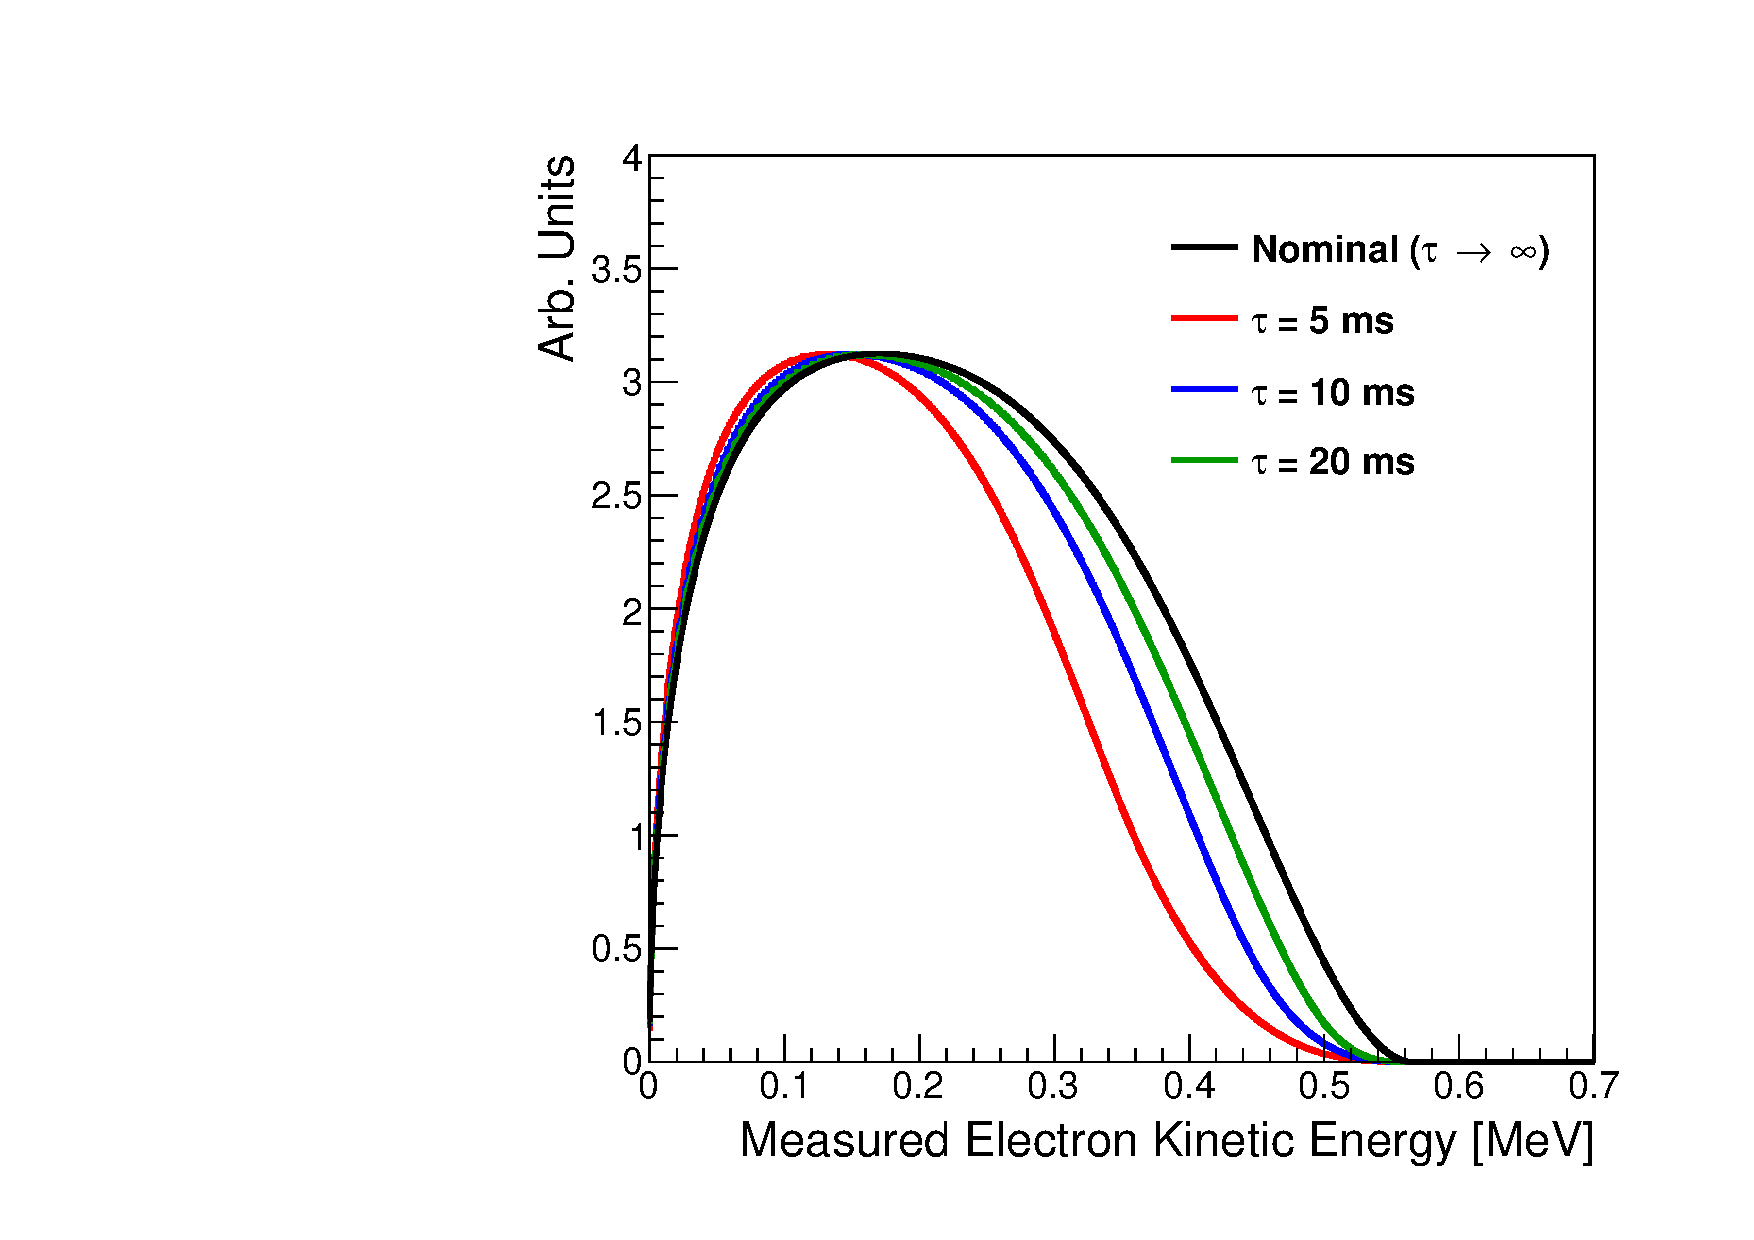
\includegraphics[width=.49\textwidth]{graphics/Ar39_energyPlot_DUNESPFD_lifetime.pdf}
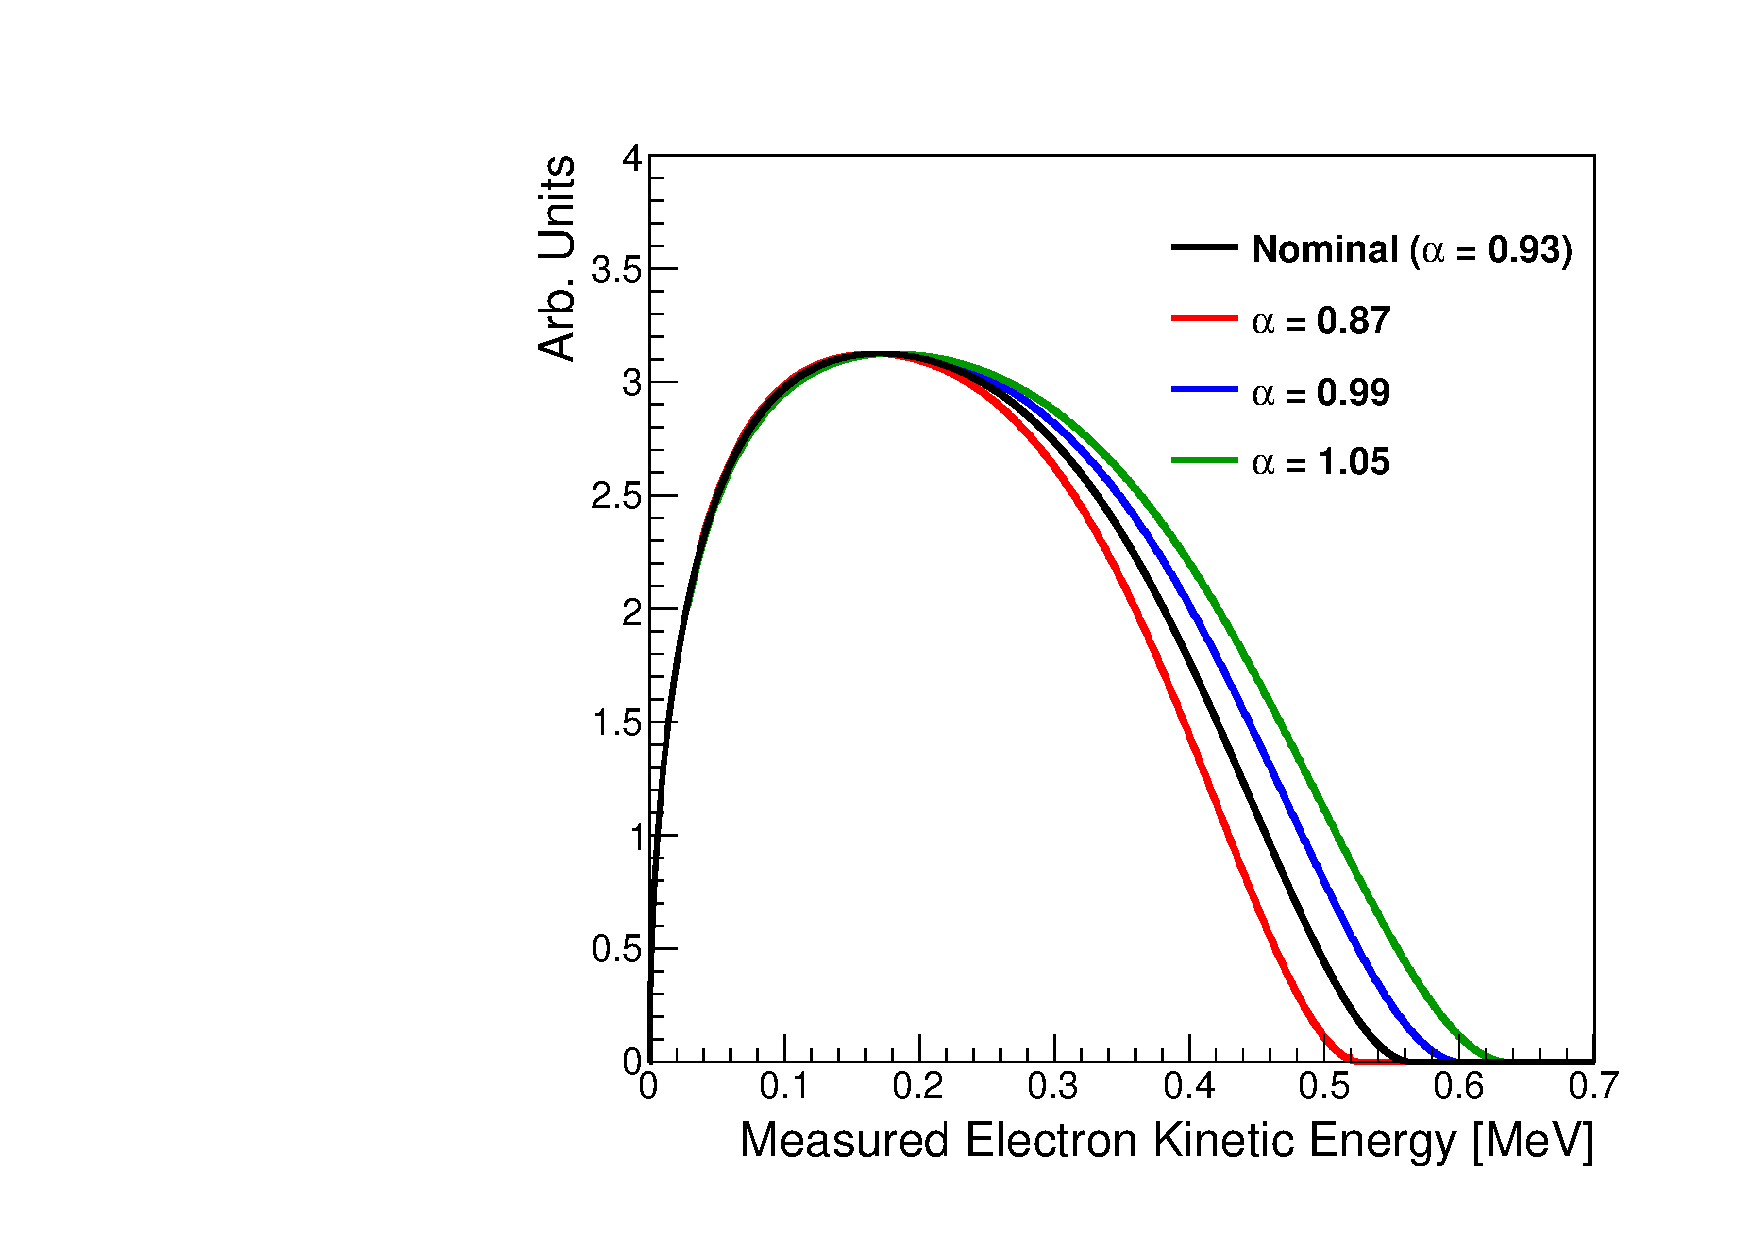
\includegraphics[width=.49\textwidth]{graphics/Ar39_energyPlot_DUNESPFD_recomb.pdf}
\end{dunefigure}